% backtracking worksheet template
\documentclass[leqno, 12pt]{article}
\usepackage{tikz}
\usetikzlibrary{positioning}
\usetikzlibrary {arrows.meta}
\usepackage[a4paper, portrait, margin=1cm]{geometry}
\usepackage{multicol}
\usepackage{fancyhdr}

\tikzset{backtrack/.style={rectangle,draw=black,fill=white,
inner sep=2pt,minimum height=32pt, minimum width=20mm}}
\tikzset{backtrackeq/.style={rectangle,draw=black,fill=white,
inner sep=2pt,minimum height=12pt, minimum width=20mm}}
\tikzset{backtrackstep/.style={rectangle,draw=none,fill=white,
inner sep=2pt,minimum height=12pt, minimum width=20mm}}

\def \HeadingAnswers {\section*{\Large Name: \underline{\hspace{8cm}} \hfill Date: \underline{\hspace{3cm}}} \vspace{-3mm}
{2-step backtracking: Answers} \vspace{1pt}\hrule}

% raise footer with page number; no header
\fancypagestyle{myfancypagestyle}{
  \fancyhf{}% clear all header and footer fields
  \renewcommand{\headrulewidth}{0pt} % no rule under header
  \fancyfoot[C] {\thepage} \setlength{\footskip}{14.5pt} % raise page number allowed min 14.5pt
}
\pagestyle{myfancypagestyle}  % apply myfancypagestyle

\begin{document}
    \HeadingAnswers
    \vspace{-8mm}
    \begin{multicols}{2}
        \begin{equation}
    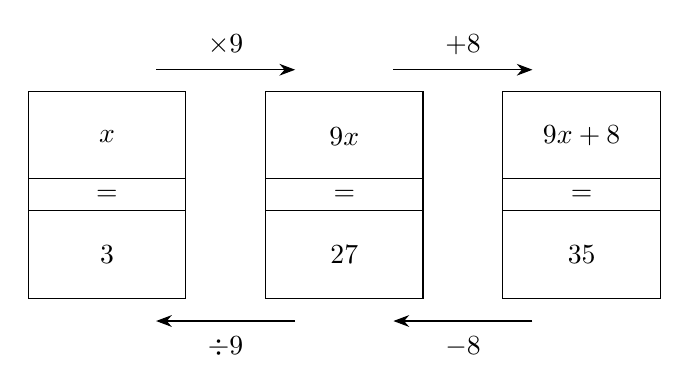
\begin{tikzpicture}[baseline={([yshift=-12pt]current bounding box.north)}]

        \node[backtrack] (boxA) at (0, 0) {$x$};
        \node[backtrack] (boxB) [right=1cm of boxA] {$9x$};
        \node[backtrack] (boxC) [right=1cm of boxB] {$9x + 8$};

        \node[backtrackeq] (boxAeq) [below=-1pt of boxA] {$=$};
        \node[backtrackeq] (boxBeq) [below=-1pt of boxB] {$=$};
        \node[backtrackeq] (boxCeq) [below=-1pt of boxC] {$=$};

        \node[backtrack] (boxArev) [below=-1pt of boxAeq] {$3$};
        \node[backtrack] (boxBrev) [below=-1pt of boxBeq] {$27$};
        \node[backtrack] (boxCrev) [below=-1pt of boxCeq] {$35$};

        \node (boxAr) at ([yshift=24pt,xshift=5mm]boxA) { };
        \node (boxBl) at ([yshift=24pt,xshift=-5mm]boxB) { };
        \draw [line width=0.4pt,-{Stealth[length=2mm]}] (boxAr)  --node[backtrackstep, above=3.0pt] {$\times9$} (boxBl);

        \node (boxBr) at ([yshift=24pt,xshift=5mm]boxB) { };
        \node (boxCl) at ([yshift=24pt,xshift=-5mm]boxC) { };
        \draw [line width=0.4pt,-{Stealth[length=2mm]}] (boxBr)  --node[backtrackstep, above=3.0pt] {$+8$} (boxCl);

        \node (boxCrevl) at ([yshift=-24pt,xshift=-5mm]boxCrev) { };
        \node (boxBrevr) at ([yshift=-24pt,xshift=5mm]boxBrev) { };
        \draw [line width=0.4pt,-{Stealth[length=2mm]}] (boxCrevl)  --node[backtrackstep, below=3.0pt] {$-8$} (boxBrevr);

        \node (boxBrevl) at ([yshift=-24pt,xshift=-5mm]boxBrev) { };
        \node (boxArevr) at ([yshift=-24pt,xshift=5mm]boxArev) { };
        \draw [line width=0.4pt,-{Stealth[length=2mm]}] (boxBrevl)  --node[backtrackstep, below=3.0pt] {$\div9$} (boxArevr);

    \end{tikzpicture}
\end{equation}


\vspace{-2pt}\begin{equation}
    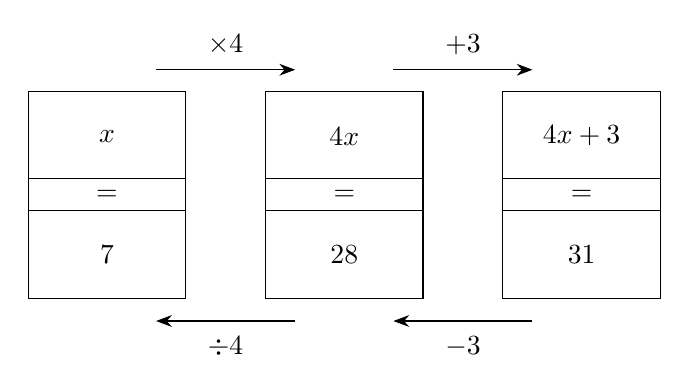
\begin{tikzpicture}[baseline={([yshift=-12pt]current bounding box.north)}]

        \node[backtrack] (boxA) at (0, 0) {$x$};
        \node[backtrack] (boxB) [right=1cm of boxA] {$4x$};
        \node[backtrack] (boxC) [right=1cm of boxB] {$4x + 3$};

        \node[backtrackeq] (boxAeq) [below=-1pt of boxA] {$=$};
        \node[backtrackeq] (boxBeq) [below=-1pt of boxB] {$=$};
        \node[backtrackeq] (boxCeq) [below=-1pt of boxC] {$=$};

        \node[backtrack] (boxArev) [below=-1pt of boxAeq] {$7$};
        \node[backtrack] (boxBrev) [below=-1pt of boxBeq] {$28$};
        \node[backtrack] (boxCrev) [below=-1pt of boxCeq] {$31$};

        \node (boxAr) at ([yshift=24pt,xshift=5mm]boxA) { };
        \node (boxBl) at ([yshift=24pt,xshift=-5mm]boxB) { };
        \draw [line width=0.4pt,-{Stealth[length=2mm]}] (boxAr)  --node[backtrackstep, above=3.0pt] {$\times4$} (boxBl);

        \node (boxBr) at ([yshift=24pt,xshift=5mm]boxB) { };
        \node (boxCl) at ([yshift=24pt,xshift=-5mm]boxC) { };
        \draw [line width=0.4pt,-{Stealth[length=2mm]}] (boxBr)  --node[backtrackstep, above=3.0pt] {$+3$} (boxCl);

        \node (boxCrevl) at ([yshift=-24pt,xshift=-5mm]boxCrev) { };
        \node (boxBrevr) at ([yshift=-24pt,xshift=5mm]boxBrev) { };
        \draw [line width=0.4pt,-{Stealth[length=2mm]}] (boxCrevl)  --node[backtrackstep, below=3.0pt] {$-3$} (boxBrevr);

        \node (boxBrevl) at ([yshift=-24pt,xshift=-5mm]boxBrev) { };
        \node (boxArevr) at ([yshift=-24pt,xshift=5mm]boxArev) { };
        \draw [line width=0.4pt,-{Stealth[length=2mm]}] (boxBrevl)  --node[backtrackstep, below=3.0pt] {$\div4$} (boxArevr);

    \end{tikzpicture}
\end{equation}


\vspace{-2pt}\begin{equation}
    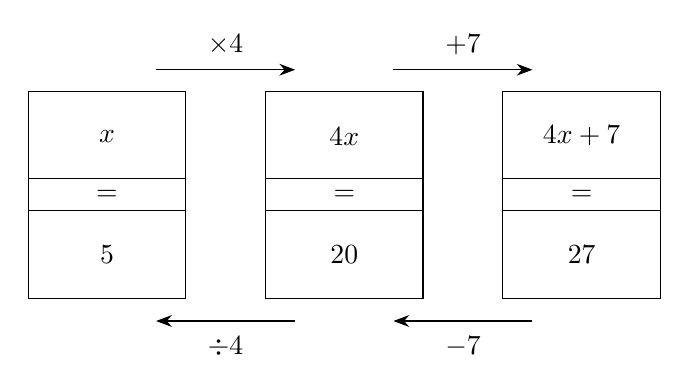
\begin{tikzpicture}[baseline={([yshift=-12pt]current bounding box.north)}]

        \node[backtrack] (boxA) at (0, 0) {$x$};
        \node[backtrack] (boxB) [right=1cm of boxA] {$4x$};
        \node[backtrack] (boxC) [right=1cm of boxB] {$4x + 7$};

        \node[backtrackeq] (boxAeq) [below=-1pt of boxA] {$=$};
        \node[backtrackeq] (boxBeq) [below=-1pt of boxB] {$=$};
        \node[backtrackeq] (boxCeq) [below=-1pt of boxC] {$=$};

        \node[backtrack] (boxArev) [below=-1pt of boxAeq] {$5$};
        \node[backtrack] (boxBrev) [below=-1pt of boxBeq] {$20$};
        \node[backtrack] (boxCrev) [below=-1pt of boxCeq] {$27$};

        \node (boxAr) at ([yshift=24pt,xshift=5mm]boxA) { };
        \node (boxBl) at ([yshift=24pt,xshift=-5mm]boxB) { };
        \draw [line width=0.4pt,-{Stealth[length=2mm]}] (boxAr)  --node[backtrackstep, above=3.0pt] {$\times4$} (boxBl);

        \node (boxBr) at ([yshift=24pt,xshift=5mm]boxB) { };
        \node (boxCl) at ([yshift=24pt,xshift=-5mm]boxC) { };
        \draw [line width=0.4pt,-{Stealth[length=2mm]}] (boxBr)  --node[backtrackstep, above=3.0pt] {$+7$} (boxCl);

        \node (boxCrevl) at ([yshift=-24pt,xshift=-5mm]boxCrev) { };
        \node (boxBrevr) at ([yshift=-24pt,xshift=5mm]boxBrev) { };
        \draw [line width=0.4pt,-{Stealth[length=2mm]}] (boxCrevl)  --node[backtrackstep, below=3.0pt] {$-7$} (boxBrevr);

        \node (boxBrevl) at ([yshift=-24pt,xshift=-5mm]boxBrev) { };
        \node (boxArevr) at ([yshift=-24pt,xshift=5mm]boxArev) { };
        \draw [line width=0.4pt,-{Stealth[length=2mm]}] (boxBrevl)  --node[backtrackstep, below=3.0pt] {$\div4$} (boxArevr);

    \end{tikzpicture}
\end{equation}


\vspace{-2pt}\begin{equation}
    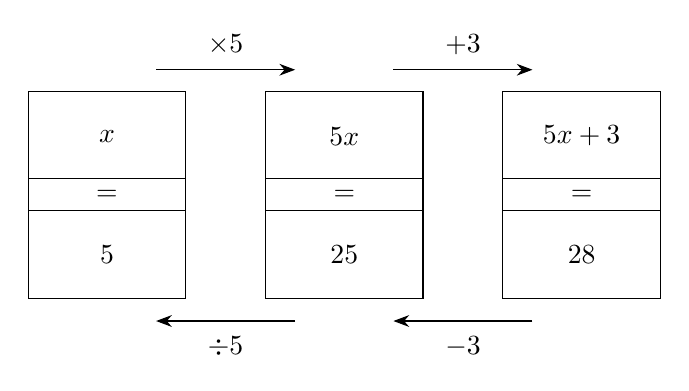
\begin{tikzpicture}[baseline={([yshift=-12pt]current bounding box.north)}]

        \node[backtrack] (boxA) at (0, 0) {$x$};
        \node[backtrack] (boxB) [right=1cm of boxA] {$5x$};
        \node[backtrack] (boxC) [right=1cm of boxB] {$5x + 3$};

        \node[backtrackeq] (boxAeq) [below=-1pt of boxA] {$=$};
        \node[backtrackeq] (boxBeq) [below=-1pt of boxB] {$=$};
        \node[backtrackeq] (boxCeq) [below=-1pt of boxC] {$=$};

        \node[backtrack] (boxArev) [below=-1pt of boxAeq] {$5$};
        \node[backtrack] (boxBrev) [below=-1pt of boxBeq] {$25$};
        \node[backtrack] (boxCrev) [below=-1pt of boxCeq] {$28$};

        \node (boxAr) at ([yshift=24pt,xshift=5mm]boxA) { };
        \node (boxBl) at ([yshift=24pt,xshift=-5mm]boxB) { };
        \draw [line width=0.4pt,-{Stealth[length=2mm]}] (boxAr)  --node[backtrackstep, above=3.0pt] {$\times5$} (boxBl);

        \node (boxBr) at ([yshift=24pt,xshift=5mm]boxB) { };
        \node (boxCl) at ([yshift=24pt,xshift=-5mm]boxC) { };
        \draw [line width=0.4pt,-{Stealth[length=2mm]}] (boxBr)  --node[backtrackstep, above=3.0pt] {$+3$} (boxCl);

        \node (boxCrevl) at ([yshift=-24pt,xshift=-5mm]boxCrev) { };
        \node (boxBrevr) at ([yshift=-24pt,xshift=5mm]boxBrev) { };
        \draw [line width=0.4pt,-{Stealth[length=2mm]}] (boxCrevl)  --node[backtrackstep, below=3.0pt] {$-3$} (boxBrevr);

        \node (boxBrevl) at ([yshift=-24pt,xshift=-5mm]boxBrev) { };
        \node (boxArevr) at ([yshift=-24pt,xshift=5mm]boxArev) { };
        \draw [line width=0.4pt,-{Stealth[length=2mm]}] (boxBrevl)  --node[backtrackstep, below=3.0pt] {$\div5$} (boxArevr);

    \end{tikzpicture}
\end{equation}


\vspace{-2pt}\begin{equation}
    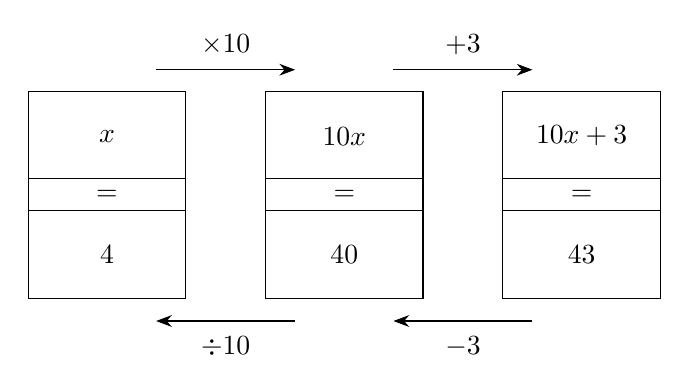
\begin{tikzpicture}[baseline={([yshift=-12pt]current bounding box.north)}]

        \node[backtrack] (boxA) at (0, 0) {$x$};
        \node[backtrack] (boxB) [right=1cm of boxA] {$10x$};
        \node[backtrack] (boxC) [right=1cm of boxB] {$10x + 3$};

        \node[backtrackeq] (boxAeq) [below=-1pt of boxA] {$=$};
        \node[backtrackeq] (boxBeq) [below=-1pt of boxB] {$=$};
        \node[backtrackeq] (boxCeq) [below=-1pt of boxC] {$=$};

        \node[backtrack] (boxArev) [below=-1pt of boxAeq] {$4$};
        \node[backtrack] (boxBrev) [below=-1pt of boxBeq] {$40$};
        \node[backtrack] (boxCrev) [below=-1pt of boxCeq] {$43$};

        \node (boxAr) at ([yshift=24pt,xshift=5mm]boxA) { };
        \node (boxBl) at ([yshift=24pt,xshift=-5mm]boxB) { };
        \draw [line width=0.4pt,-{Stealth[length=2mm]}] (boxAr)  --node[backtrackstep, above=3.0pt] {$\times10$} (boxBl);

        \node (boxBr) at ([yshift=24pt,xshift=5mm]boxB) { };
        \node (boxCl) at ([yshift=24pt,xshift=-5mm]boxC) { };
        \draw [line width=0.4pt,-{Stealth[length=2mm]}] (boxBr)  --node[backtrackstep, above=3.0pt] {$+3$} (boxCl);

        \node (boxCrevl) at ([yshift=-24pt,xshift=-5mm]boxCrev) { };
        \node (boxBrevr) at ([yshift=-24pt,xshift=5mm]boxBrev) { };
        \draw [line width=0.4pt,-{Stealth[length=2mm]}] (boxCrevl)  --node[backtrackstep, below=3.0pt] {$-3$} (boxBrevr);

        \node (boxBrevl) at ([yshift=-24pt,xshift=-5mm]boxBrev) { };
        \node (boxArevr) at ([yshift=-24pt,xshift=5mm]boxArev) { };
        \draw [line width=0.4pt,-{Stealth[length=2mm]}] (boxBrevl)  --node[backtrackstep, below=3.0pt] {$\div10$} (boxArevr);

    \end{tikzpicture}
\end{equation}


\vspace{-2pt}\begin{equation}
    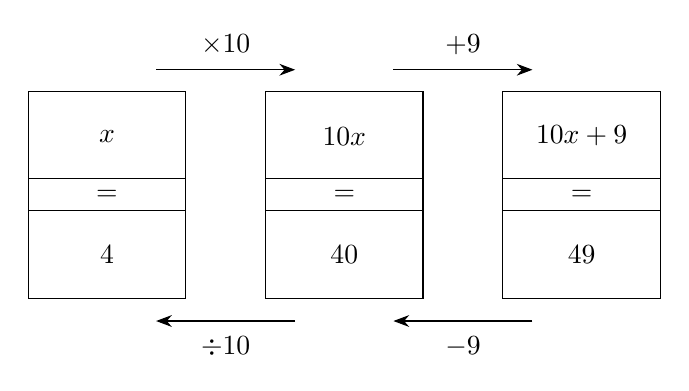
\begin{tikzpicture}[baseline={([yshift=-12pt]current bounding box.north)}]

        \node[backtrack] (boxA) at (0, 0) {$x$};
        \node[backtrack] (boxB) [right=1cm of boxA] {$10x$};
        \node[backtrack] (boxC) [right=1cm of boxB] {$10x + 9$};

        \node[backtrackeq] (boxAeq) [below=-1pt of boxA] {$=$};
        \node[backtrackeq] (boxBeq) [below=-1pt of boxB] {$=$};
        \node[backtrackeq] (boxCeq) [below=-1pt of boxC] {$=$};

        \node[backtrack] (boxArev) [below=-1pt of boxAeq] {$4$};
        \node[backtrack] (boxBrev) [below=-1pt of boxBeq] {$40$};
        \node[backtrack] (boxCrev) [below=-1pt of boxCeq] {$49$};

        \node (boxAr) at ([yshift=24pt,xshift=5mm]boxA) { };
        \node (boxBl) at ([yshift=24pt,xshift=-5mm]boxB) { };
        \draw [line width=0.4pt,-{Stealth[length=2mm]}] (boxAr)  --node[backtrackstep, above=3.0pt] {$\times10$} (boxBl);

        \node (boxBr) at ([yshift=24pt,xshift=5mm]boxB) { };
        \node (boxCl) at ([yshift=24pt,xshift=-5mm]boxC) { };
        \draw [line width=0.4pt,-{Stealth[length=2mm]}] (boxBr)  --node[backtrackstep, above=3.0pt] {$+9$} (boxCl);

        \node (boxCrevl) at ([yshift=-24pt,xshift=-5mm]boxCrev) { };
        \node (boxBrevr) at ([yshift=-24pt,xshift=5mm]boxBrev) { };
        \draw [line width=0.4pt,-{Stealth[length=2mm]}] (boxCrevl)  --node[backtrackstep, below=3.0pt] {$-9$} (boxBrevr);

        \node (boxBrevl) at ([yshift=-24pt,xshift=-5mm]boxBrev) { };
        \node (boxArevr) at ([yshift=-24pt,xshift=5mm]boxArev) { };
        \draw [line width=0.4pt,-{Stealth[length=2mm]}] (boxBrevl)  --node[backtrackstep, below=3.0pt] {$\div10$} (boxArevr);

    \end{tikzpicture}
\end{equation}


\vspace{-2pt}\begin{equation}
    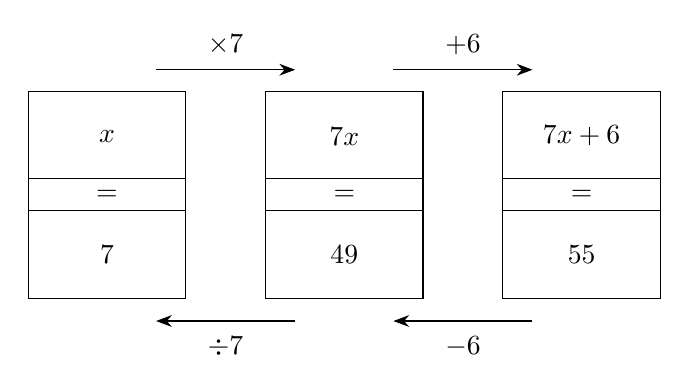
\begin{tikzpicture}[baseline={([yshift=-12pt]current bounding box.north)}]

        \node[backtrack] (boxA) at (0, 0) {$x$};
        \node[backtrack] (boxB) [right=1cm of boxA] {$7x$};
        \node[backtrack] (boxC) [right=1cm of boxB] {$7x + 6$};

        \node[backtrackeq] (boxAeq) [below=-1pt of boxA] {$=$};
        \node[backtrackeq] (boxBeq) [below=-1pt of boxB] {$=$};
        \node[backtrackeq] (boxCeq) [below=-1pt of boxC] {$=$};

        \node[backtrack] (boxArev) [below=-1pt of boxAeq] {$7$};
        \node[backtrack] (boxBrev) [below=-1pt of boxBeq] {$49$};
        \node[backtrack] (boxCrev) [below=-1pt of boxCeq] {$55$};

        \node (boxAr) at ([yshift=24pt,xshift=5mm]boxA) { };
        \node (boxBl) at ([yshift=24pt,xshift=-5mm]boxB) { };
        \draw [line width=0.4pt,-{Stealth[length=2mm]}] (boxAr)  --node[backtrackstep, above=3.0pt] {$\times7$} (boxBl);

        \node (boxBr) at ([yshift=24pt,xshift=5mm]boxB) { };
        \node (boxCl) at ([yshift=24pt,xshift=-5mm]boxC) { };
        \draw [line width=0.4pt,-{Stealth[length=2mm]}] (boxBr)  --node[backtrackstep, above=3.0pt] {$+6$} (boxCl);

        \node (boxCrevl) at ([yshift=-24pt,xshift=-5mm]boxCrev) { };
        \node (boxBrevr) at ([yshift=-24pt,xshift=5mm]boxBrev) { };
        \draw [line width=0.4pt,-{Stealth[length=2mm]}] (boxCrevl)  --node[backtrackstep, below=3.0pt] {$-6$} (boxBrevr);

        \node (boxBrevl) at ([yshift=-24pt,xshift=-5mm]boxBrev) { };
        \node (boxArevr) at ([yshift=-24pt,xshift=5mm]boxArev) { };
        \draw [line width=0.4pt,-{Stealth[length=2mm]}] (boxBrevl)  --node[backtrackstep, below=3.0pt] {$\div7$} (boxArevr);

    \end{tikzpicture}
\end{equation}


\vspace{-2pt}\begin{equation}
    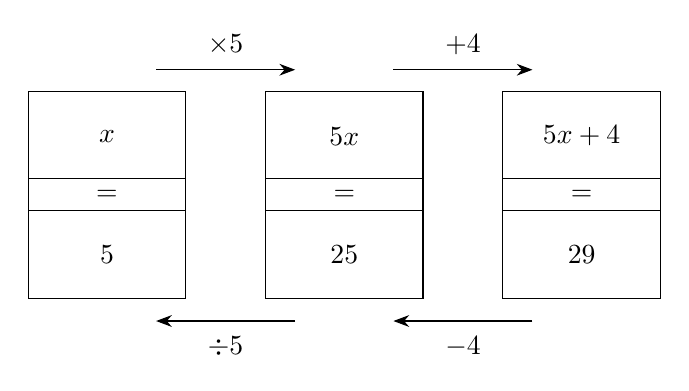
\begin{tikzpicture}[baseline={([yshift=-12pt]current bounding box.north)}]

        \node[backtrack] (boxA) at (0, 0) {$x$};
        \node[backtrack] (boxB) [right=1cm of boxA] {$5x$};
        \node[backtrack] (boxC) [right=1cm of boxB] {$5x + 4$};

        \node[backtrackeq] (boxAeq) [below=-1pt of boxA] {$=$};
        \node[backtrackeq] (boxBeq) [below=-1pt of boxB] {$=$};
        \node[backtrackeq] (boxCeq) [below=-1pt of boxC] {$=$};

        \node[backtrack] (boxArev) [below=-1pt of boxAeq] {$5$};
        \node[backtrack] (boxBrev) [below=-1pt of boxBeq] {$25$};
        \node[backtrack] (boxCrev) [below=-1pt of boxCeq] {$29$};

        \node (boxAr) at ([yshift=24pt,xshift=5mm]boxA) { };
        \node (boxBl) at ([yshift=24pt,xshift=-5mm]boxB) { };
        \draw [line width=0.4pt,-{Stealth[length=2mm]}] (boxAr)  --node[backtrackstep, above=3.0pt] {$\times5$} (boxBl);

        \node (boxBr) at ([yshift=24pt,xshift=5mm]boxB) { };
        \node (boxCl) at ([yshift=24pt,xshift=-5mm]boxC) { };
        \draw [line width=0.4pt,-{Stealth[length=2mm]}] (boxBr)  --node[backtrackstep, above=3.0pt] {$+4$} (boxCl);

        \node (boxCrevl) at ([yshift=-24pt,xshift=-5mm]boxCrev) { };
        \node (boxBrevr) at ([yshift=-24pt,xshift=5mm]boxBrev) { };
        \draw [line width=0.4pt,-{Stealth[length=2mm]}] (boxCrevl)  --node[backtrackstep, below=3.0pt] {$-4$} (boxBrevr);

        \node (boxBrevl) at ([yshift=-24pt,xshift=-5mm]boxBrev) { };
        \node (boxArevr) at ([yshift=-24pt,xshift=5mm]boxArev) { };
        \draw [line width=0.4pt,-{Stealth[length=2mm]}] (boxBrevl)  --node[backtrackstep, below=3.0pt] {$\div5$} (boxArevr);

    \end{tikzpicture}
\end{equation}


\vspace{-2pt}\begin{equation}
    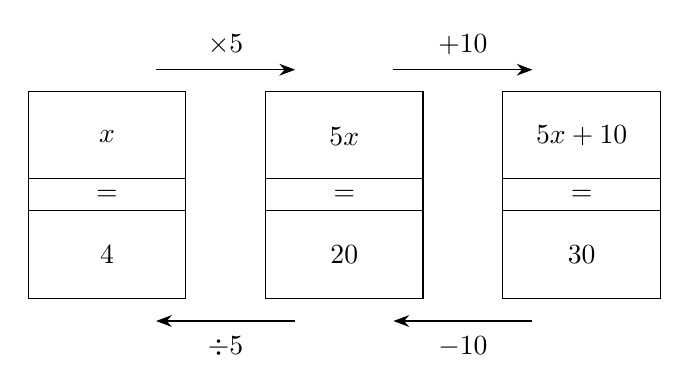
\begin{tikzpicture}[baseline={([yshift=-12pt]current bounding box.north)}]

        \node[backtrack] (boxA) at (0, 0) {$x$};
        \node[backtrack] (boxB) [right=1cm of boxA] {$5x$};
        \node[backtrack] (boxC) [right=1cm of boxB] {$5x + 10$};

        \node[backtrackeq] (boxAeq) [below=-1pt of boxA] {$=$};
        \node[backtrackeq] (boxBeq) [below=-1pt of boxB] {$=$};
        \node[backtrackeq] (boxCeq) [below=-1pt of boxC] {$=$};

        \node[backtrack] (boxArev) [below=-1pt of boxAeq] {$4$};
        \node[backtrack] (boxBrev) [below=-1pt of boxBeq] {$20$};
        \node[backtrack] (boxCrev) [below=-1pt of boxCeq] {$30$};

        \node (boxAr) at ([yshift=24pt,xshift=5mm]boxA) { };
        \node (boxBl) at ([yshift=24pt,xshift=-5mm]boxB) { };
        \draw [line width=0.4pt,-{Stealth[length=2mm]}] (boxAr)  --node[backtrackstep, above=3.0pt] {$\times5$} (boxBl);

        \node (boxBr) at ([yshift=24pt,xshift=5mm]boxB) { };
        \node (boxCl) at ([yshift=24pt,xshift=-5mm]boxC) { };
        \draw [line width=0.4pt,-{Stealth[length=2mm]}] (boxBr)  --node[backtrackstep, above=3.0pt] {$+10$} (boxCl);

        \node (boxCrevl) at ([yshift=-24pt,xshift=-5mm]boxCrev) { };
        \node (boxBrevr) at ([yshift=-24pt,xshift=5mm]boxBrev) { };
        \draw [line width=0.4pt,-{Stealth[length=2mm]}] (boxCrevl)  --node[backtrackstep, below=3.0pt] {$-10$} (boxBrevr);

        \node (boxBrevl) at ([yshift=-24pt,xshift=-5mm]boxBrev) { };
        \node (boxArevr) at ([yshift=-24pt,xshift=5mm]boxArev) { };
        \draw [line width=0.4pt,-{Stealth[length=2mm]}] (boxBrevl)  --node[backtrackstep, below=3.0pt] {$\div5$} (boxArevr);

    \end{tikzpicture}
\end{equation}


\vspace{-2pt}\begin{equation}
    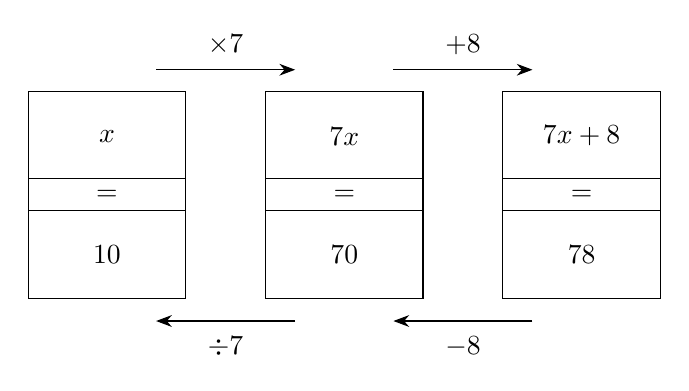
\begin{tikzpicture}[baseline={([yshift=-12pt]current bounding box.north)}]

        \node[backtrack] (boxA) at (0, 0) {$x$};
        \node[backtrack] (boxB) [right=1cm of boxA] {$7x$};
        \node[backtrack] (boxC) [right=1cm of boxB] {$7x + 8$};

        \node[backtrackeq] (boxAeq) [below=-1pt of boxA] {$=$};
        \node[backtrackeq] (boxBeq) [below=-1pt of boxB] {$=$};
        \node[backtrackeq] (boxCeq) [below=-1pt of boxC] {$=$};

        \node[backtrack] (boxArev) [below=-1pt of boxAeq] {$10$};
        \node[backtrack] (boxBrev) [below=-1pt of boxBeq] {$70$};
        \node[backtrack] (boxCrev) [below=-1pt of boxCeq] {$78$};

        \node (boxAr) at ([yshift=24pt,xshift=5mm]boxA) { };
        \node (boxBl) at ([yshift=24pt,xshift=-5mm]boxB) { };
        \draw [line width=0.4pt,-{Stealth[length=2mm]}] (boxAr)  --node[backtrackstep, above=3.0pt] {$\times7$} (boxBl);

        \node (boxBr) at ([yshift=24pt,xshift=5mm]boxB) { };
        \node (boxCl) at ([yshift=24pt,xshift=-5mm]boxC) { };
        \draw [line width=0.4pt,-{Stealth[length=2mm]}] (boxBr)  --node[backtrackstep, above=3.0pt] {$+8$} (boxCl);

        \node (boxCrevl) at ([yshift=-24pt,xshift=-5mm]boxCrev) { };
        \node (boxBrevr) at ([yshift=-24pt,xshift=5mm]boxBrev) { };
        \draw [line width=0.4pt,-{Stealth[length=2mm]}] (boxCrevl)  --node[backtrackstep, below=3.0pt] {$-8$} (boxBrevr);

        \node (boxBrevl) at ([yshift=-24pt,xshift=-5mm]boxBrev) { };
        \node (boxArevr) at ([yshift=-24pt,xshift=5mm]boxArev) { };
        \draw [line width=0.4pt,-{Stealth[length=2mm]}] (boxBrevl)  --node[backtrackstep, below=3.0pt] {$\div7$} (boxArevr);

    \end{tikzpicture}
\end{equation}


\vspace{-2pt}\begin{equation}
    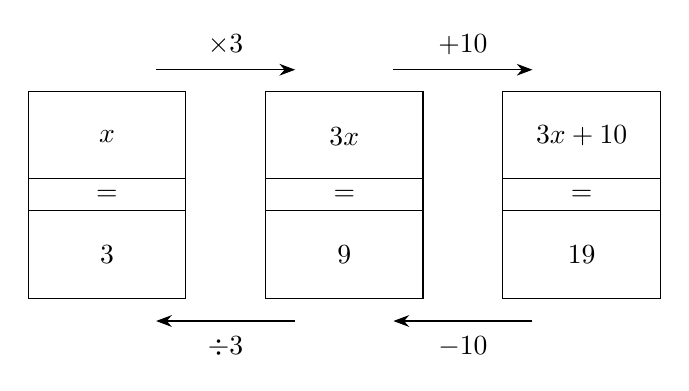
\begin{tikzpicture}[baseline={([yshift=-12pt]current bounding box.north)}]

        \node[backtrack] (boxA) at (0, 0) {$x$};
        \node[backtrack] (boxB) [right=1cm of boxA] {$3x$};
        \node[backtrack] (boxC) [right=1cm of boxB] {$3x + 10$};

        \node[backtrackeq] (boxAeq) [below=-1pt of boxA] {$=$};
        \node[backtrackeq] (boxBeq) [below=-1pt of boxB] {$=$};
        \node[backtrackeq] (boxCeq) [below=-1pt of boxC] {$=$};

        \node[backtrack] (boxArev) [below=-1pt of boxAeq] {$3$};
        \node[backtrack] (boxBrev) [below=-1pt of boxBeq] {$9$};
        \node[backtrack] (boxCrev) [below=-1pt of boxCeq] {$19$};

        \node (boxAr) at ([yshift=24pt,xshift=5mm]boxA) { };
        \node (boxBl) at ([yshift=24pt,xshift=-5mm]boxB) { };
        \draw [line width=0.4pt,-{Stealth[length=2mm]}] (boxAr)  --node[backtrackstep, above=3.0pt] {$\times3$} (boxBl);

        \node (boxBr) at ([yshift=24pt,xshift=5mm]boxB) { };
        \node (boxCl) at ([yshift=24pt,xshift=-5mm]boxC) { };
        \draw [line width=0.4pt,-{Stealth[length=2mm]}] (boxBr)  --node[backtrackstep, above=3.0pt] {$+10$} (boxCl);

        \node (boxCrevl) at ([yshift=-24pt,xshift=-5mm]boxCrev) { };
        \node (boxBrevr) at ([yshift=-24pt,xshift=5mm]boxBrev) { };
        \draw [line width=0.4pt,-{Stealth[length=2mm]}] (boxCrevl)  --node[backtrackstep, below=3.0pt] {$-10$} (boxBrevr);

        \node (boxBrevl) at ([yshift=-24pt,xshift=-5mm]boxBrev) { };
        \node (boxArevr) at ([yshift=-24pt,xshift=5mm]boxArev) { };
        \draw [line width=0.4pt,-{Stealth[length=2mm]}] (boxBrevl)  --node[backtrackstep, below=3.0pt] {$\div3$} (boxArevr);

    \end{tikzpicture}
\end{equation}


\vspace{-2pt}\begin{equation}
    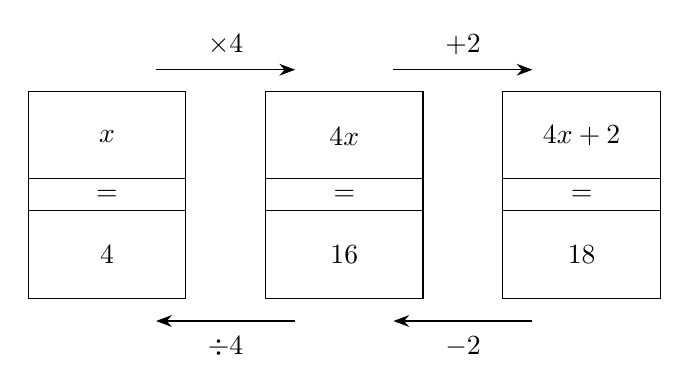
\begin{tikzpicture}[baseline={([yshift=-12pt]current bounding box.north)}]

        \node[backtrack] (boxA) at (0, 0) {$x$};
        \node[backtrack] (boxB) [right=1cm of boxA] {$4x$};
        \node[backtrack] (boxC) [right=1cm of boxB] {$4x + 2$};

        \node[backtrackeq] (boxAeq) [below=-1pt of boxA] {$=$};
        \node[backtrackeq] (boxBeq) [below=-1pt of boxB] {$=$};
        \node[backtrackeq] (boxCeq) [below=-1pt of boxC] {$=$};

        \node[backtrack] (boxArev) [below=-1pt of boxAeq] {$4$};
        \node[backtrack] (boxBrev) [below=-1pt of boxBeq] {$16$};
        \node[backtrack] (boxCrev) [below=-1pt of boxCeq] {$18$};

        \node (boxAr) at ([yshift=24pt,xshift=5mm]boxA) { };
        \node (boxBl) at ([yshift=24pt,xshift=-5mm]boxB) { };
        \draw [line width=0.4pt,-{Stealth[length=2mm]}] (boxAr)  --node[backtrackstep, above=3.0pt] {$\times4$} (boxBl);

        \node (boxBr) at ([yshift=24pt,xshift=5mm]boxB) { };
        \node (boxCl) at ([yshift=24pt,xshift=-5mm]boxC) { };
        \draw [line width=0.4pt,-{Stealth[length=2mm]}] (boxBr)  --node[backtrackstep, above=3.0pt] {$+2$} (boxCl);

        \node (boxCrevl) at ([yshift=-24pt,xshift=-5mm]boxCrev) { };
        \node (boxBrevr) at ([yshift=-24pt,xshift=5mm]boxBrev) { };
        \draw [line width=0.4pt,-{Stealth[length=2mm]}] (boxCrevl)  --node[backtrackstep, below=3.0pt] {$-2$} (boxBrevr);

        \node (boxBrevl) at ([yshift=-24pt,xshift=-5mm]boxBrev) { };
        \node (boxArevr) at ([yshift=-24pt,xshift=5mm]boxArev) { };
        \draw [line width=0.4pt,-{Stealth[length=2mm]}] (boxBrevl)  --node[backtrackstep, below=3.0pt] {$\div4$} (boxArevr);

    \end{tikzpicture}
\end{equation}


\vspace{-2pt}\begin{equation}
    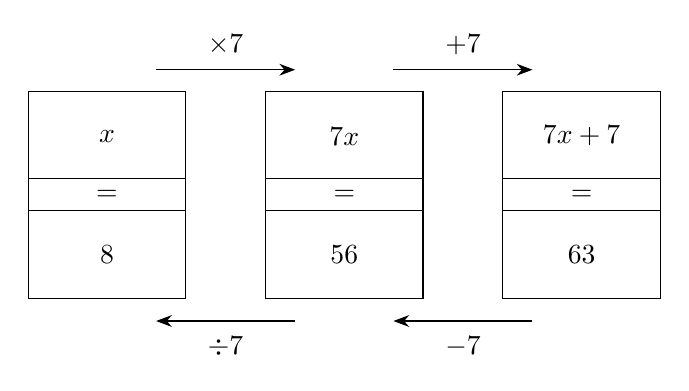
\begin{tikzpicture}[baseline={([yshift=-12pt]current bounding box.north)}]

        \node[backtrack] (boxA) at (0, 0) {$x$};
        \node[backtrack] (boxB) [right=1cm of boxA] {$7x$};
        \node[backtrack] (boxC) [right=1cm of boxB] {$7x + 7$};

        \node[backtrackeq] (boxAeq) [below=-1pt of boxA] {$=$};
        \node[backtrackeq] (boxBeq) [below=-1pt of boxB] {$=$};
        \node[backtrackeq] (boxCeq) [below=-1pt of boxC] {$=$};

        \node[backtrack] (boxArev) [below=-1pt of boxAeq] {$8$};
        \node[backtrack] (boxBrev) [below=-1pt of boxBeq] {$56$};
        \node[backtrack] (boxCrev) [below=-1pt of boxCeq] {$63$};

        \node (boxAr) at ([yshift=24pt,xshift=5mm]boxA) { };
        \node (boxBl) at ([yshift=24pt,xshift=-5mm]boxB) { };
        \draw [line width=0.4pt,-{Stealth[length=2mm]}] (boxAr)  --node[backtrackstep, above=3.0pt] {$\times7$} (boxBl);

        \node (boxBr) at ([yshift=24pt,xshift=5mm]boxB) { };
        \node (boxCl) at ([yshift=24pt,xshift=-5mm]boxC) { };
        \draw [line width=0.4pt,-{Stealth[length=2mm]}] (boxBr)  --node[backtrackstep, above=3.0pt] {$+7$} (boxCl);

        \node (boxCrevl) at ([yshift=-24pt,xshift=-5mm]boxCrev) { };
        \node (boxBrevr) at ([yshift=-24pt,xshift=5mm]boxBrev) { };
        \draw [line width=0.4pt,-{Stealth[length=2mm]}] (boxCrevl)  --node[backtrackstep, below=3.0pt] {$-7$} (boxBrevr);

        \node (boxBrevl) at ([yshift=-24pt,xshift=-5mm]boxBrev) { };
        \node (boxArevr) at ([yshift=-24pt,xshift=5mm]boxArev) { };
        \draw [line width=0.4pt,-{Stealth[length=2mm]}] (boxBrevl)  --node[backtrackstep, below=3.0pt] {$\div7$} (boxArevr);

    \end{tikzpicture}
\end{equation}


\vspace{-2pt}\begin{equation}
    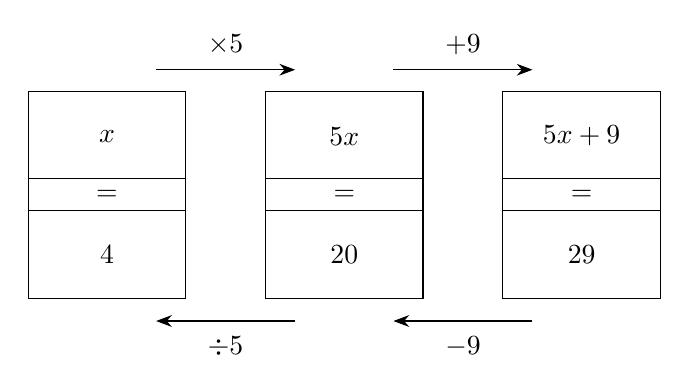
\begin{tikzpicture}[baseline={([yshift=-12pt]current bounding box.north)}]

        \node[backtrack] (boxA) at (0, 0) {$x$};
        \node[backtrack] (boxB) [right=1cm of boxA] {$5x$};
        \node[backtrack] (boxC) [right=1cm of boxB] {$5x + 9$};

        \node[backtrackeq] (boxAeq) [below=-1pt of boxA] {$=$};
        \node[backtrackeq] (boxBeq) [below=-1pt of boxB] {$=$};
        \node[backtrackeq] (boxCeq) [below=-1pt of boxC] {$=$};

        \node[backtrack] (boxArev) [below=-1pt of boxAeq] {$4$};
        \node[backtrack] (boxBrev) [below=-1pt of boxBeq] {$20$};
        \node[backtrack] (boxCrev) [below=-1pt of boxCeq] {$29$};

        \node (boxAr) at ([yshift=24pt,xshift=5mm]boxA) { };
        \node (boxBl) at ([yshift=24pt,xshift=-5mm]boxB) { };
        \draw [line width=0.4pt,-{Stealth[length=2mm]}] (boxAr)  --node[backtrackstep, above=3.0pt] {$\times5$} (boxBl);

        \node (boxBr) at ([yshift=24pt,xshift=5mm]boxB) { };
        \node (boxCl) at ([yshift=24pt,xshift=-5mm]boxC) { };
        \draw [line width=0.4pt,-{Stealth[length=2mm]}] (boxBr)  --node[backtrackstep, above=3.0pt] {$+9$} (boxCl);

        \node (boxCrevl) at ([yshift=-24pt,xshift=-5mm]boxCrev) { };
        \node (boxBrevr) at ([yshift=-24pt,xshift=5mm]boxBrev) { };
        \draw [line width=0.4pt,-{Stealth[length=2mm]}] (boxCrevl)  --node[backtrackstep, below=3.0pt] {$-9$} (boxBrevr);

        \node (boxBrevl) at ([yshift=-24pt,xshift=-5mm]boxBrev) { };
        \node (boxArevr) at ([yshift=-24pt,xshift=5mm]boxArev) { };
        \draw [line width=0.4pt,-{Stealth[length=2mm]}] (boxBrevl)  --node[backtrackstep, below=3.0pt] {$\div5$} (boxArevr);

    \end{tikzpicture}
\end{equation}


\vspace{-2pt}\begin{equation}
    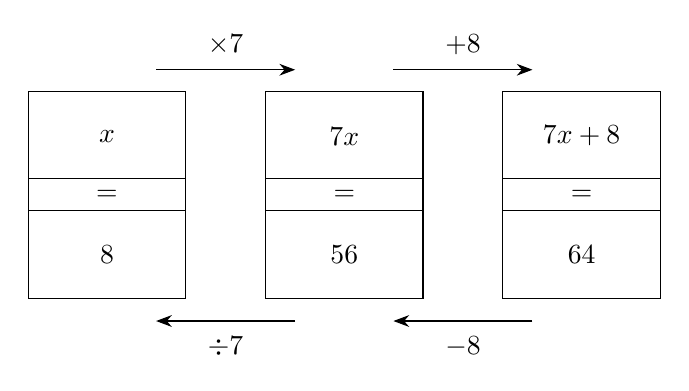
\begin{tikzpicture}[baseline={([yshift=-12pt]current bounding box.north)}]

        \node[backtrack] (boxA) at (0, 0) {$x$};
        \node[backtrack] (boxB) [right=1cm of boxA] {$7x$};
        \node[backtrack] (boxC) [right=1cm of boxB] {$7x + 8$};

        \node[backtrackeq] (boxAeq) [below=-1pt of boxA] {$=$};
        \node[backtrackeq] (boxBeq) [below=-1pt of boxB] {$=$};
        \node[backtrackeq] (boxCeq) [below=-1pt of boxC] {$=$};

        \node[backtrack] (boxArev) [below=-1pt of boxAeq] {$8$};
        \node[backtrack] (boxBrev) [below=-1pt of boxBeq] {$56$};
        \node[backtrack] (boxCrev) [below=-1pt of boxCeq] {$64$};

        \node (boxAr) at ([yshift=24pt,xshift=5mm]boxA) { };
        \node (boxBl) at ([yshift=24pt,xshift=-5mm]boxB) { };
        \draw [line width=0.4pt,-{Stealth[length=2mm]}] (boxAr)  --node[backtrackstep, above=3.0pt] {$\times7$} (boxBl);

        \node (boxBr) at ([yshift=24pt,xshift=5mm]boxB) { };
        \node (boxCl) at ([yshift=24pt,xshift=-5mm]boxC) { };
        \draw [line width=0.4pt,-{Stealth[length=2mm]}] (boxBr)  --node[backtrackstep, above=3.0pt] {$+8$} (boxCl);

        \node (boxCrevl) at ([yshift=-24pt,xshift=-5mm]boxCrev) { };
        \node (boxBrevr) at ([yshift=-24pt,xshift=5mm]boxBrev) { };
        \draw [line width=0.4pt,-{Stealth[length=2mm]}] (boxCrevl)  --node[backtrackstep, below=3.0pt] {$-8$} (boxBrevr);

        \node (boxBrevl) at ([yshift=-24pt,xshift=-5mm]boxBrev) { };
        \node (boxArevr) at ([yshift=-24pt,xshift=5mm]boxArev) { };
        \draw [line width=0.4pt,-{Stealth[length=2mm]}] (boxBrevl)  --node[backtrackstep, below=3.0pt] {$\div7$} (boxArevr);

    \end{tikzpicture}
\end{equation}


\vspace{-2pt}\begin{equation}
    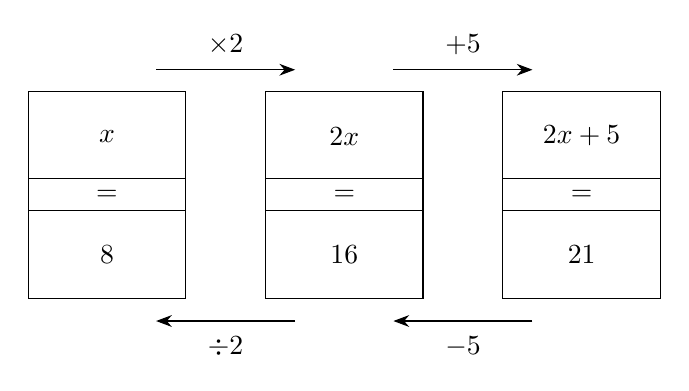
\begin{tikzpicture}[baseline={([yshift=-12pt]current bounding box.north)}]

        \node[backtrack] (boxA) at (0, 0) {$x$};
        \node[backtrack] (boxB) [right=1cm of boxA] {$2x$};
        \node[backtrack] (boxC) [right=1cm of boxB] {$2x + 5$};

        \node[backtrackeq] (boxAeq) [below=-1pt of boxA] {$=$};
        \node[backtrackeq] (boxBeq) [below=-1pt of boxB] {$=$};
        \node[backtrackeq] (boxCeq) [below=-1pt of boxC] {$=$};

        \node[backtrack] (boxArev) [below=-1pt of boxAeq] {$8$};
        \node[backtrack] (boxBrev) [below=-1pt of boxBeq] {$16$};
        \node[backtrack] (boxCrev) [below=-1pt of boxCeq] {$21$};

        \node (boxAr) at ([yshift=24pt,xshift=5mm]boxA) { };
        \node (boxBl) at ([yshift=24pt,xshift=-5mm]boxB) { };
        \draw [line width=0.4pt,-{Stealth[length=2mm]}] (boxAr)  --node[backtrackstep, above=3.0pt] {$\times2$} (boxBl);

        \node (boxBr) at ([yshift=24pt,xshift=5mm]boxB) { };
        \node (boxCl) at ([yshift=24pt,xshift=-5mm]boxC) { };
        \draw [line width=0.4pt,-{Stealth[length=2mm]}] (boxBr)  --node[backtrackstep, above=3.0pt] {$+5$} (boxCl);

        \node (boxCrevl) at ([yshift=-24pt,xshift=-5mm]boxCrev) { };
        \node (boxBrevr) at ([yshift=-24pt,xshift=5mm]boxBrev) { };
        \draw [line width=0.4pt,-{Stealth[length=2mm]}] (boxCrevl)  --node[backtrackstep, below=3.0pt] {$-5$} (boxBrevr);

        \node (boxBrevl) at ([yshift=-24pt,xshift=-5mm]boxBrev) { };
        \node (boxArevr) at ([yshift=-24pt,xshift=5mm]boxArev) { };
        \draw [line width=0.4pt,-{Stealth[length=2mm]}] (boxBrevl)  --node[backtrackstep, below=3.0pt] {$\div2$} (boxArevr);

    \end{tikzpicture}
\end{equation}


\vspace{-2pt}\begin{equation}
    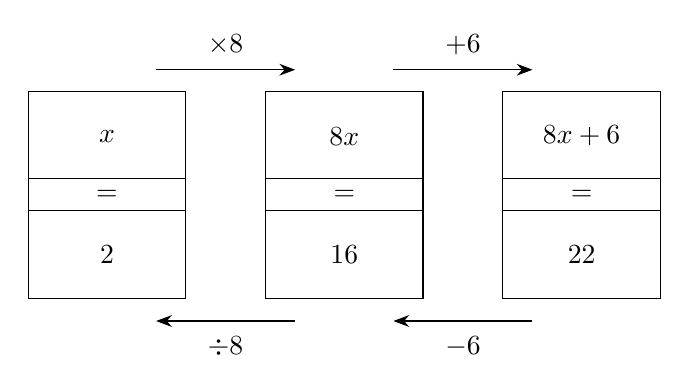
\begin{tikzpicture}[baseline={([yshift=-12pt]current bounding box.north)}]

        \node[backtrack] (boxA) at (0, 0) {$x$};
        \node[backtrack] (boxB) [right=1cm of boxA] {$8x$};
        \node[backtrack] (boxC) [right=1cm of boxB] {$8x + 6$};

        \node[backtrackeq] (boxAeq) [below=-1pt of boxA] {$=$};
        \node[backtrackeq] (boxBeq) [below=-1pt of boxB] {$=$};
        \node[backtrackeq] (boxCeq) [below=-1pt of boxC] {$=$};

        \node[backtrack] (boxArev) [below=-1pt of boxAeq] {$2$};
        \node[backtrack] (boxBrev) [below=-1pt of boxBeq] {$16$};
        \node[backtrack] (boxCrev) [below=-1pt of boxCeq] {$22$};

        \node (boxAr) at ([yshift=24pt,xshift=5mm]boxA) { };
        \node (boxBl) at ([yshift=24pt,xshift=-5mm]boxB) { };
        \draw [line width=0.4pt,-{Stealth[length=2mm]}] (boxAr)  --node[backtrackstep, above=3.0pt] {$\times8$} (boxBl);

        \node (boxBr) at ([yshift=24pt,xshift=5mm]boxB) { };
        \node (boxCl) at ([yshift=24pt,xshift=-5mm]boxC) { };
        \draw [line width=0.4pt,-{Stealth[length=2mm]}] (boxBr)  --node[backtrackstep, above=3.0pt] {$+6$} (boxCl);

        \node (boxCrevl) at ([yshift=-24pt,xshift=-5mm]boxCrev) { };
        \node (boxBrevr) at ([yshift=-24pt,xshift=5mm]boxBrev) { };
        \draw [line width=0.4pt,-{Stealth[length=2mm]}] (boxCrevl)  --node[backtrackstep, below=3.0pt] {$-6$} (boxBrevr);

        \node (boxBrevl) at ([yshift=-24pt,xshift=-5mm]boxBrev) { };
        \node (boxArevr) at ([yshift=-24pt,xshift=5mm]boxArev) { };
        \draw [line width=0.4pt,-{Stealth[length=2mm]}] (boxBrevl)  --node[backtrackstep, below=3.0pt] {$\div8$} (boxArevr);

    \end{tikzpicture}
\end{equation}


\vspace{-2pt}\begin{equation}
    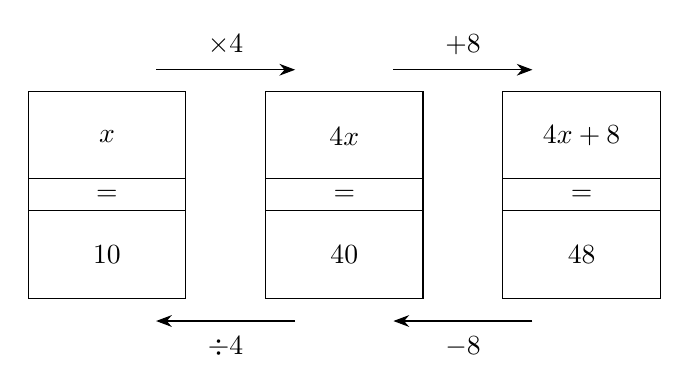
\begin{tikzpicture}[baseline={([yshift=-12pt]current bounding box.north)}]

        \node[backtrack] (boxA) at (0, 0) {$x$};
        \node[backtrack] (boxB) [right=1cm of boxA] {$4x$};
        \node[backtrack] (boxC) [right=1cm of boxB] {$4x + 8$};

        \node[backtrackeq] (boxAeq) [below=-1pt of boxA] {$=$};
        \node[backtrackeq] (boxBeq) [below=-1pt of boxB] {$=$};
        \node[backtrackeq] (boxCeq) [below=-1pt of boxC] {$=$};

        \node[backtrack] (boxArev) [below=-1pt of boxAeq] {$10$};
        \node[backtrack] (boxBrev) [below=-1pt of boxBeq] {$40$};
        \node[backtrack] (boxCrev) [below=-1pt of boxCeq] {$48$};

        \node (boxAr) at ([yshift=24pt,xshift=5mm]boxA) { };
        \node (boxBl) at ([yshift=24pt,xshift=-5mm]boxB) { };
        \draw [line width=0.4pt,-{Stealth[length=2mm]}] (boxAr)  --node[backtrackstep, above=3.0pt] {$\times4$} (boxBl);

        \node (boxBr) at ([yshift=24pt,xshift=5mm]boxB) { };
        \node (boxCl) at ([yshift=24pt,xshift=-5mm]boxC) { };
        \draw [line width=0.4pt,-{Stealth[length=2mm]}] (boxBr)  --node[backtrackstep, above=3.0pt] {$+8$} (boxCl);

        \node (boxCrevl) at ([yshift=-24pt,xshift=-5mm]boxCrev) { };
        \node (boxBrevr) at ([yshift=-24pt,xshift=5mm]boxBrev) { };
        \draw [line width=0.4pt,-{Stealth[length=2mm]}] (boxCrevl)  --node[backtrackstep, below=3.0pt] {$-8$} (boxBrevr);

        \node (boxBrevl) at ([yshift=-24pt,xshift=-5mm]boxBrev) { };
        \node (boxArevr) at ([yshift=-24pt,xshift=5mm]boxArev) { };
        \draw [line width=0.4pt,-{Stealth[length=2mm]}] (boxBrevl)  --node[backtrackstep, below=3.0pt] {$\div4$} (boxArevr);

    \end{tikzpicture}
\end{equation}


\vspace{-2pt}\begin{equation}
    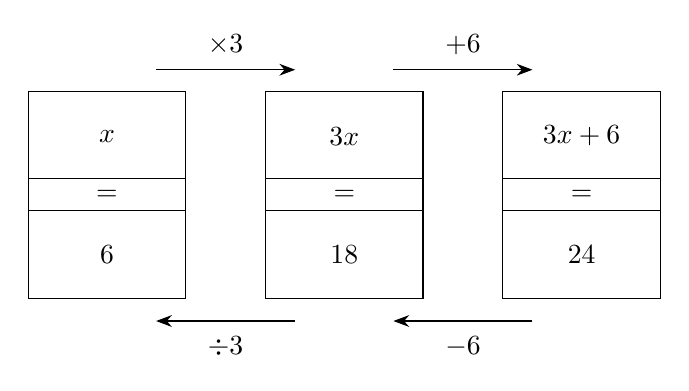
\begin{tikzpicture}[baseline={([yshift=-12pt]current bounding box.north)}]

        \node[backtrack] (boxA) at (0, 0) {$x$};
        \node[backtrack] (boxB) [right=1cm of boxA] {$3x$};
        \node[backtrack] (boxC) [right=1cm of boxB] {$3x + 6$};

        \node[backtrackeq] (boxAeq) [below=-1pt of boxA] {$=$};
        \node[backtrackeq] (boxBeq) [below=-1pt of boxB] {$=$};
        \node[backtrackeq] (boxCeq) [below=-1pt of boxC] {$=$};

        \node[backtrack] (boxArev) [below=-1pt of boxAeq] {$6$};
        \node[backtrack] (boxBrev) [below=-1pt of boxBeq] {$18$};
        \node[backtrack] (boxCrev) [below=-1pt of boxCeq] {$24$};

        \node (boxAr) at ([yshift=24pt,xshift=5mm]boxA) { };
        \node (boxBl) at ([yshift=24pt,xshift=-5mm]boxB) { };
        \draw [line width=0.4pt,-{Stealth[length=2mm]}] (boxAr)  --node[backtrackstep, above=3.0pt] {$\times3$} (boxBl);

        \node (boxBr) at ([yshift=24pt,xshift=5mm]boxB) { };
        \node (boxCl) at ([yshift=24pt,xshift=-5mm]boxC) { };
        \draw [line width=0.4pt,-{Stealth[length=2mm]}] (boxBr)  --node[backtrackstep, above=3.0pt] {$+6$} (boxCl);

        \node (boxCrevl) at ([yshift=-24pt,xshift=-5mm]boxCrev) { };
        \node (boxBrevr) at ([yshift=-24pt,xshift=5mm]boxBrev) { };
        \draw [line width=0.4pt,-{Stealth[length=2mm]}] (boxCrevl)  --node[backtrackstep, below=3.0pt] {$-6$} (boxBrevr);

        \node (boxBrevl) at ([yshift=-24pt,xshift=-5mm]boxBrev) { };
        \node (boxArevr) at ([yshift=-24pt,xshift=5mm]boxArev) { };
        \draw [line width=0.4pt,-{Stealth[length=2mm]}] (boxBrevl)  --node[backtrackstep, below=3.0pt] {$\div3$} (boxArevr);

    \end{tikzpicture}
\end{equation}


\vspace{-2pt}\begin{equation}
    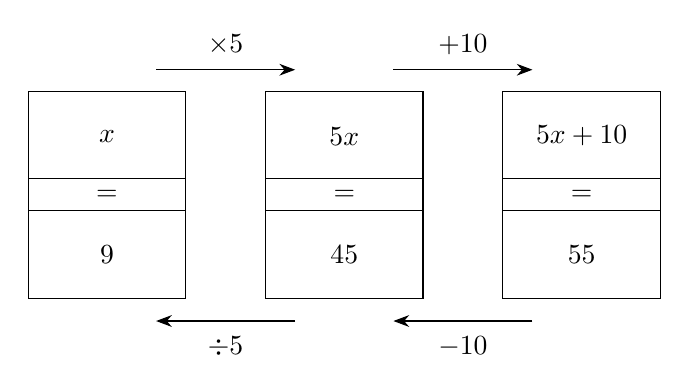
\begin{tikzpicture}[baseline={([yshift=-12pt]current bounding box.north)}]

        \node[backtrack] (boxA) at (0, 0) {$x$};
        \node[backtrack] (boxB) [right=1cm of boxA] {$5x$};
        \node[backtrack] (boxC) [right=1cm of boxB] {$5x + 10$};

        \node[backtrackeq] (boxAeq) [below=-1pt of boxA] {$=$};
        \node[backtrackeq] (boxBeq) [below=-1pt of boxB] {$=$};
        \node[backtrackeq] (boxCeq) [below=-1pt of boxC] {$=$};

        \node[backtrack] (boxArev) [below=-1pt of boxAeq] {$9$};
        \node[backtrack] (boxBrev) [below=-1pt of boxBeq] {$45$};
        \node[backtrack] (boxCrev) [below=-1pt of boxCeq] {$55$};

        \node (boxAr) at ([yshift=24pt,xshift=5mm]boxA) { };
        \node (boxBl) at ([yshift=24pt,xshift=-5mm]boxB) { };
        \draw [line width=0.4pt,-{Stealth[length=2mm]}] (boxAr)  --node[backtrackstep, above=3.0pt] {$\times5$} (boxBl);

        \node (boxBr) at ([yshift=24pt,xshift=5mm]boxB) { };
        \node (boxCl) at ([yshift=24pt,xshift=-5mm]boxC) { };
        \draw [line width=0.4pt,-{Stealth[length=2mm]}] (boxBr)  --node[backtrackstep, above=3.0pt] {$+10$} (boxCl);

        \node (boxCrevl) at ([yshift=-24pt,xshift=-5mm]boxCrev) { };
        \node (boxBrevr) at ([yshift=-24pt,xshift=5mm]boxBrev) { };
        \draw [line width=0.4pt,-{Stealth[length=2mm]}] (boxCrevl)  --node[backtrackstep, below=3.0pt] {$-10$} (boxBrevr);

        \node (boxBrevl) at ([yshift=-24pt,xshift=-5mm]boxBrev) { };
        \node (boxArevr) at ([yshift=-24pt,xshift=5mm]boxArev) { };
        \draw [line width=0.4pt,-{Stealth[length=2mm]}] (boxBrevl)  --node[backtrackstep, below=3.0pt] {$\div5$} (boxArevr);

    \end{tikzpicture}
\end{equation}


\vspace{-2pt}
    \end{multicols}
\end{document}
